\documentclass[12pt]{article}

% Page geometry -- NBER style
\usepackage[margin=1in]{geometry}

% Font: Times New Roman
\usepackage{newtxtext,newtxmath}

% Double spacing
\usepackage{setspace}
\doublespacing

% Bibliography -- author-year
\usepackage[authoryear,round]{natbib}

% Tables
\usepackage{booktabs}
\usepackage{longtable}

% Figures
\usepackage{graphicx}

% Math
\usepackage{amsmath}

% Appendices
\usepackage[titletoc]{appendix}

% Captions
\usepackage{caption}

% Hyperlinks (load last)
\usepackage[hidelinks]{hyperref}

\title{Corporate Governance Reform and the Korea Discount:\\
Evidence from Japan's Natural Experiment}
\author{[Author]}
\date{\today}

\begin{document}
\maketitle

\begin{abstract}
% ABSTRACT -- to be completed in Plan 03
Placeholder abstract.
\end{abstract}

\newpage
\tableofcontents
\newpage

\section{Introduction}
% INTRODUCTION -- to be completed in Plan 03

\section{Institutional Background}
% INSTITUTIONAL BACKGROUND -- to be completed in Plan 03

\section{Literature Review}
% LITERATURE REVIEW -- to be completed in Plan 03

\section{Data}
% DATA -- to be completed in Plan 03

\section{Causal Mechanisms}
% CAUSAL MECHANISMS -- to be completed in Plan 04

\section{Empirical Strategy}
% EMPIRICAL STRATEGY -- to be completed in Plan 04

\section{Results}
% RESULTS -- to be completed in Plan 04

% Figure 1: 20-year KOSPI P/B vs peers
\begin{figure}[htbp]
  \centering
  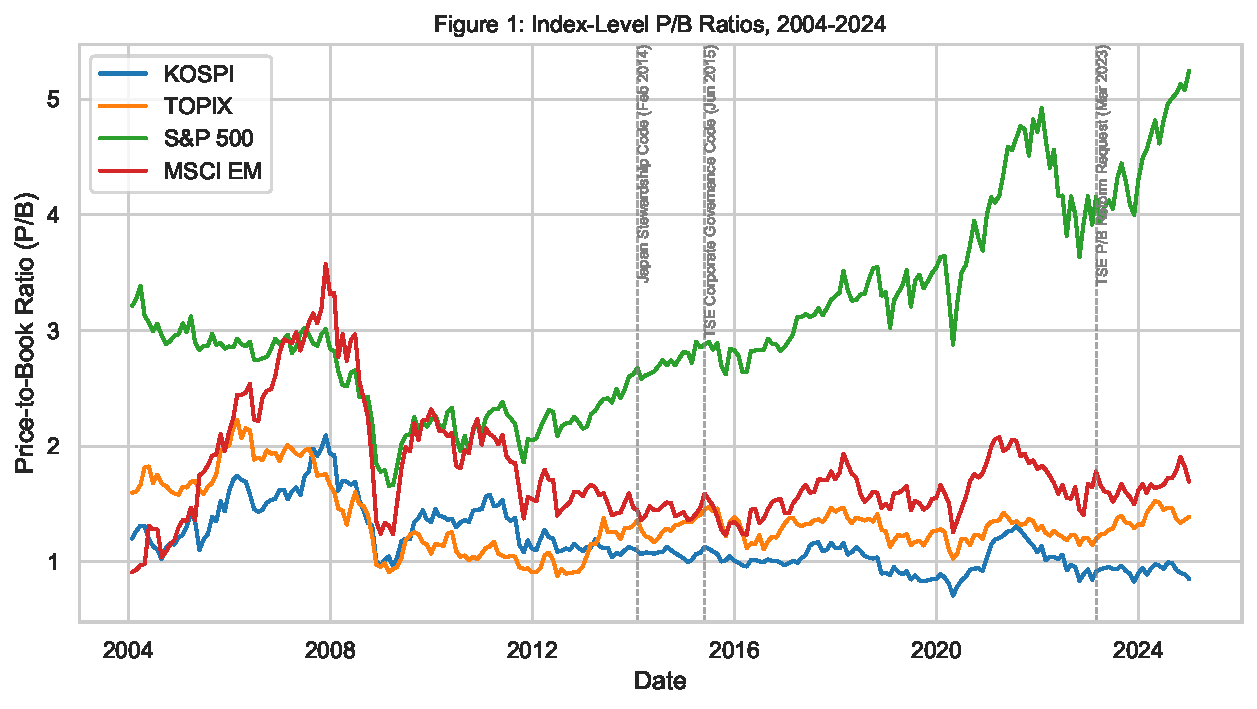
\includegraphics[width=\textwidth]{../output/figures/figure1_pb_comparison.pdf}
  \caption{KOSPI P/B ratio relative to TOPIX, S\&P 500, and MSCI EM (2004--2024).}
  \label{fig:pb_comparison}
\end{figure}

% Figure 2: Stacked event study CARs
\begin{figure}[htbp]
  \centering
  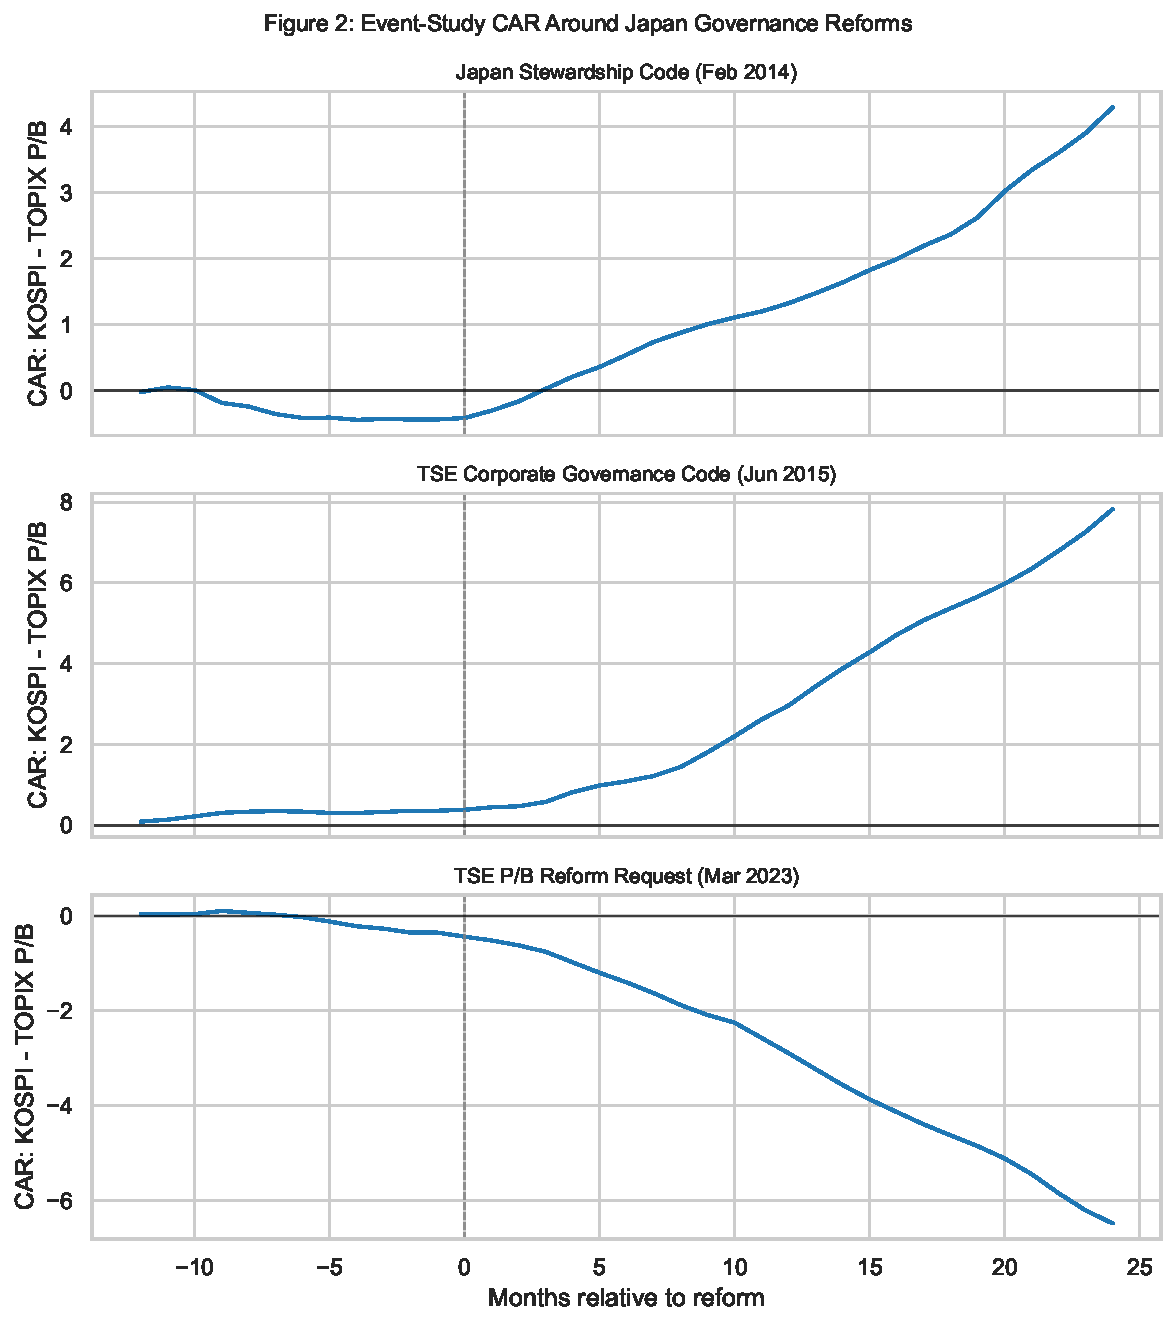
\includegraphics[width=\textwidth]{../output/figures/figure2_event_study.pdf}
  \caption{Cumulative abnormal valuation changes around Japan's three corporate governance reform dates.}
  \label{fig:event_study}
\end{figure}

% Table 1: Summary statistics
\begin{table}
\caption{Summary statistics of index-level P/B ratios by country and sub-period.}
\label{tab:summary_stats}
\begin{tabular}{llrrrrr}
\toprule
 & Period & mean & median & std & min & max \\
country &  &  &  &  &  &  \\
\midrule
KOSPI & Full (2004--2024) & 1.18 & 1.10 & 0.26 & 0.71 & 2.09 \\
MSCI\_EM & Full (2004--2024) & 1.78 & 1.65 & 0.47 & 0.91 & 3.58 \\
SP500 & Full (2004--2024) & 3.08 & 2.89 & 0.81 & 1.66 & 5.25 \\
TOPIX & Full (2004--2024) & 1.35 & 1.31 & 0.28 & 0.88 & 2.23 \\
KOSPI & Pre-reform (2004--2013) & 1.36 & 1.34 & 0.25 & 0.96 & 2.09 \\
MSCI\_EM & Pre-reform (2004--2013) & 1.97 & 1.91 & 0.60 & 0.91 & 3.58 \\
SP500 & Pre-reform (2004--2013) & 2.51 & 2.42 & 0.40 & 1.66 & 3.39 \\
TOPIX & Pre-reform (2004--2013) & 1.41 & 1.29 & 0.39 & 0.88 & 2.23 \\
KOSPI & Reform era (2014--2022) & 1.02 & 1.03 & 0.12 & 0.71 & 1.31 \\
MSCI\_EM & Reform era (2014--2022) & 1.59 & 1.55 & 0.20 & 1.24 & 2.08 \\
SP500 & Reform era (2014--2022) & 3.39 & 3.28 & 0.63 & 2.58 & 4.92 \\
TOPIX & Reform era (2014--2022) & 1.29 & 1.28 & 0.10 & 1.03 & 1.48 \\
KOSPI & Post-TSE (2023--2024) & 0.93 & 0.94 & 0.04 & 0.83 & 1.00 \\
MSCI\_EM & Post-TSE (2023--2024) & 1.66 & 1.66 & 0.10 & 1.50 & 1.91 \\
SP500 & Post-TSE (2023--2024) & 4.51 & 4.47 & 0.43 & 3.91 & 5.25 \\
TOPIX & Post-TSE (2023--2024) & 1.36 & 1.35 & 0.10 & 1.15 & 1.53 \\
\bottomrule
\end{tabular}
\end{table}


% Table 2: Panel OLS with wild-bootstrap p-values
\begin{table}
\caption{Two-way fixed effects PanelOLS estimates of Japan reform valuation responses.}
\label{tab:panel_ols}
\begin{tabular}{llll}
\toprule
 & Baseline two-way FE & + reform dummies & + reform x Japan \\
term &  &  &  \\
\midrule
post\_stewardship &  & absorbed by time FE & absorbed by time FE \\
post\_cgc &  & absorbed by time FE & absorbed by time FE \\
post\_tse\_pb\_reform &  & absorbed by time FE & absorbed by time FE \\
stewardship\_x\_japan &  &  & 0.09 [0.625] \\
cgc\_x\_japan &  &  & -0.32 [0.375] \\
tse\_pb\_reform\_x\_japan &  &  & -0.23 [0.500] \\
log\_fx & -0.02 (0.01) & -0.02 (0.01) & -0.01 (0.01) \\
\multicolumn{4}{l}{\footnotesize Note: Coefficients from two-way FE PanelOLS. For \textit{+ reform x Japan} specification, bracketed values are wild-bootstrap p-values (999 Rademacher draws, clustered by country). Standard errors shown for all other estimable cells.} \\
\bottomrule
\end{tabular}
\end{table}


% Event study coefficient table
% Descriptive CARs: coefficients and cumulative abnormal KOSPI-TOPIX P/B spread.
% Standard errors are not reported: the saturated cohort x relative-time design
% makes sandwich robust inference undefined. See paper text for robustness discussion.
\begin{table}
\caption{Stacked event-study descriptive CAR estimates (no inference reported).}
\label{tab:event_study_coefs}
\begin{tabular}{lrrr}
\toprule
Event & Month & Coefficient & CAR \\
\midrule
Japan Stewardship Code (Feb 2014) & -12 & -0.02 & -0.02 \\
Japan Stewardship Code (Feb 2014) & -11 & 0.07 & 0.05 \\
Japan Stewardship Code (Feb 2014) & -10 & -0.04 & 0.01 \\
Japan Stewardship Code (Feb 2014) & -9 & -0.19 & -0.19 \\
Japan Stewardship Code (Feb 2014) & -8 & -0.06 & -0.24 \\
Japan Stewardship Code (Feb 2014) & -7 & -0.11 & -0.36 \\
Japan Stewardship Code (Feb 2014) & -6 & -0.06 & -0.42 \\
Japan Stewardship Code (Feb 2014) & -5 & 0.00 & -0.41 \\
Japan Stewardship Code (Feb 2014) & -4 & -0.03 & -0.44 \\
Japan Stewardship Code (Feb 2014) & -3 & 0.01 & -0.43 \\
Japan Stewardship Code (Feb 2014) & -2 & -0.01 & -0.44 \\
Japan Stewardship Code (Feb 2014) & -1 & 0.00 & -0.44 \\
Japan Stewardship Code (Feb 2014) & 0 & 0.02 & -0.42 \\
Japan Stewardship Code (Feb 2014) & 1 & 0.11 & -0.30 \\
Japan Stewardship Code (Feb 2014) & 2 & 0.14 & -0.17 \\
Japan Stewardship Code (Feb 2014) & 3 & 0.19 & 0.02 \\
Japan Stewardship Code (Feb 2014) & 4 & 0.18 & 0.21 \\
Japan Stewardship Code (Feb 2014) & 5 & 0.15 & 0.36 \\
Japan Stewardship Code (Feb 2014) & 6 & 0.18 & 0.54 \\
Japan Stewardship Code (Feb 2014) & 7 & 0.19 & 0.74 \\
Japan Stewardship Code (Feb 2014) & 8 & 0.14 & 0.88 \\
Japan Stewardship Code (Feb 2014) & 9 & 0.13 & 1.00 \\
Japan Stewardship Code (Feb 2014) & 10 & 0.10 & 1.11 \\
Japan Stewardship Code (Feb 2014) & 11 & 0.09 & 1.20 \\
Japan Stewardship Code (Feb 2014) & 12 & 0.12 & 1.32 \\
Japan Stewardship Code (Feb 2014) & 13 & 0.15 & 1.47 \\
Japan Stewardship Code (Feb 2014) & 14 & 0.16 & 1.64 \\
Japan Stewardship Code (Feb 2014) & 15 & 0.19 & 1.82 \\
Japan Stewardship Code (Feb 2014) & 16 & 0.16 & 1.99 \\
Japan Stewardship Code (Feb 2014) & 17 & 0.20 & 2.19 \\
Japan Stewardship Code (Feb 2014) & 18 & 0.17 & 2.36 \\
Japan Stewardship Code (Feb 2014) & 19 & 0.26 & 2.62 \\
Japan Stewardship Code (Feb 2014) & 20 & 0.40 & 3.02 \\
Japan Stewardship Code (Feb 2014) & 21 & 0.32 & 3.34 \\
Japan Stewardship Code (Feb 2014) & 22 & 0.26 & 3.60 \\
Japan Stewardship Code (Feb 2014) & 23 & 0.30 & 3.90 \\
Japan Stewardship Code (Feb 2014) & 24 & 0.39 & 4.29 \\
TSE Corporate Governance Code (Jun 2015) & -12 & 0.09 & 0.09 \\
TSE Corporate Governance Code (Jun 2015) & -11 & 0.05 & 0.14 \\
TSE Corporate Governance Code (Jun 2015) & -10 & 0.08 & 0.22 \\
TSE Corporate Governance Code (Jun 2015) & -9 & 0.09 & 0.31 \\
TSE Corporate Governance Code (Jun 2015) & -8 & 0.03 & 0.33 \\
TSE Corporate Governance Code (Jun 2015) & -7 & 0.01 & 0.35 \\
TSE Corporate Governance Code (Jun 2015) & -6 & -0.01 & 0.33 \\
TSE Corporate Governance Code (Jun 2015) & -5 & -0.03 & 0.30 \\
TSE Corporate Governance Code (Jun 2015) & -4 & -0.00 & 0.30 \\
TSE Corporate Governance Code (Jun 2015) & -3 & 0.02 & 0.33 \\
TSE Corporate Governance Code (Jun 2015) & -2 & 0.03 & 0.36 \\
TSE Corporate Governance Code (Jun 2015) & -1 & 0.00 & 0.36 \\
TSE Corporate Governance Code (Jun 2015) & 0 & 0.03 & 0.38 \\
TSE Corporate Governance Code (Jun 2015) & 1 & 0.06 & 0.44 \\
TSE Corporate Governance Code (Jun 2015) & 2 & 0.03 & 0.47 \\
TSE Corporate Governance Code (Jun 2015) & 3 & 0.11 & 0.58 \\
TSE Corporate Governance Code (Jun 2015) & 4 & 0.24 & 0.82 \\
TSE Corporate Governance Code (Jun 2015) & 5 & 0.16 & 0.98 \\
TSE Corporate Governance Code (Jun 2015) & 6 & 0.10 & 1.09 \\
TSE Corporate Governance Code (Jun 2015) & 7 & 0.13 & 1.22 \\
TSE Corporate Governance Code (Jun 2015) & 8 & 0.22 & 1.44 \\
TSE Corporate Governance Code (Jun 2015) & 9 & 0.37 & 1.81 \\
TSE Corporate Governance Code (Jun 2015) & 10 & 0.40 & 2.20 \\
TSE Corporate Governance Code (Jun 2015) & 11 & 0.42 & 2.62 \\
TSE Corporate Governance Code (Jun 2015) & 12 & 0.34 & 2.97 \\
TSE Corporate Governance Code (Jun 2015) & 13 & 0.47 & 3.44 \\
TSE Corporate Governance Code (Jun 2015) & 14 & 0.44 & 3.88 \\
TSE Corporate Governance Code (Jun 2015) & 15 & 0.40 & 4.28 \\
TSE Corporate Governance Code (Jun 2015) & 16 & 0.43 & 4.71 \\
TSE Corporate Governance Code (Jun 2015) & 17 & 0.36 & 5.08 \\
TSE Corporate Governance Code (Jun 2015) & 18 & 0.30 & 5.37 \\
TSE Corporate Governance Code (Jun 2015) & 19 & 0.29 & 5.66 \\
TSE Corporate Governance Code (Jun 2015) & 20 & 0.32 & 5.98 \\
TSE Corporate Governance Code (Jun 2015) & 21 & 0.37 & 6.35 \\
TSE Corporate Governance Code (Jun 2015) & 22 & 0.45 & 6.80 \\
TSE Corporate Governance Code (Jun 2015) & 23 & 0.47 & 7.26 \\
TSE Corporate Governance Code (Jun 2015) & 24 & 0.57 & 7.83 \\
TSE P/B Reform Request (Mar 2023) & -12 & 0.03 & 0.03 \\
TSE P/B Reform Request (Mar 2023) & -11 & -0.00 & 0.03 \\
TSE P/B Reform Request (Mar 2023) & -10 & 0.01 & 0.04 \\
TSE P/B Reform Request (Mar 2023) & -9 & 0.07 & 0.11 \\
TSE P/B Reform Request (Mar 2023) & -8 & -0.04 & 0.07 \\
TSE P/B Reform Request (Mar 2023) & -7 & -0.04 & 0.03 \\
TSE P/B Reform Request (Mar 2023) & -6 & -0.05 & -0.03 \\
TSE P/B Reform Request (Mar 2023) & -5 & -0.09 & -0.12 \\
TSE P/B Reform Request (Mar 2023) & -4 & -0.10 & -0.22 \\
TSE P/B Reform Request (Mar 2023) & -3 & -0.05 & -0.27 \\
TSE P/B Reform Request (Mar 2023) & -2 & -0.08 & -0.35 \\
TSE P/B Reform Request (Mar 2023) & -1 & 0.00 & -0.35 \\
TSE P/B Reform Request (Mar 2023) & 0 & -0.08 & -0.44 \\
TSE P/B Reform Request (Mar 2023) & 1 & -0.08 & -0.52 \\
TSE P/B Reform Request (Mar 2023) & 2 & -0.10 & -0.62 \\
TSE P/B Reform Request (Mar 2023) & 3 & -0.13 & -0.75 \\
TSE P/B Reform Request (Mar 2023) & 4 & -0.22 & -0.98 \\
TSE P/B Reform Request (Mar 2023) & 5 & -0.22 & -1.20 \\
TSE P/B Reform Request (Mar 2023) & 6 & -0.20 & -1.40 \\
TSE P/B Reform Request (Mar 2023) & 7 & -0.22 & -1.63 \\
TSE P/B Reform Request (Mar 2023) & 8 & -0.25 & -1.88 \\
TSE P/B Reform Request (Mar 2023) & 9 & -0.21 & -2.09 \\
TSE P/B Reform Request (Mar 2023) & 10 & -0.16 & -2.25 \\
TSE P/B Reform Request (Mar 2023) & 11 & -0.32 & -2.57 \\
TSE P/B Reform Request (Mar 2023) & 12 & -0.32 & -2.89 \\
TSE P/B Reform Request (Mar 2023) & 13 & -0.34 & -3.23 \\
TSE P/B Reform Request (Mar 2023) & 14 & -0.33 & -3.56 \\
TSE P/B Reform Request (Mar 2023) & 15 & -0.30 & -3.87 \\
TSE P/B Reform Request (Mar 2023) & 16 & -0.26 & -4.13 \\
TSE P/B Reform Request (Mar 2023) & 17 & -0.26 & -4.39 \\
TSE P/B Reform Request (Mar 2023) & 18 & -0.23 & -4.63 \\
TSE P/B Reform Request (Mar 2023) & 19 & -0.23 & -4.85 \\
TSE P/B Reform Request (Mar 2023) & 20 & -0.26 & -5.11 \\
TSE P/B Reform Request (Mar 2023) & 21 & -0.33 & -5.44 \\
TSE P/B Reform Request (Mar 2023) & 22 & -0.40 & -5.85 \\
TSE P/B Reform Request (Mar 2023) & 23 & -0.36 & -6.21 \\
TSE P/B Reform Request (Mar 2023) & 24 & -0.27 & -6.48 \\
\bottomrule
\end{tabular}
\end{table}


\section{Discussion and Limitations}
% DISCUSSION AND LIMITATIONS -- to be completed in Plan 04

\section{Conclusion}
% CONCLUSION -- to be completed in Plan 04

\section{Policy Recommendations}
% POLICY RECOMMENDATIONS -- to be completed in Plan 04

% Figure 4: Counterfactual projection
\begin{figure}[htbp]
  \centering
  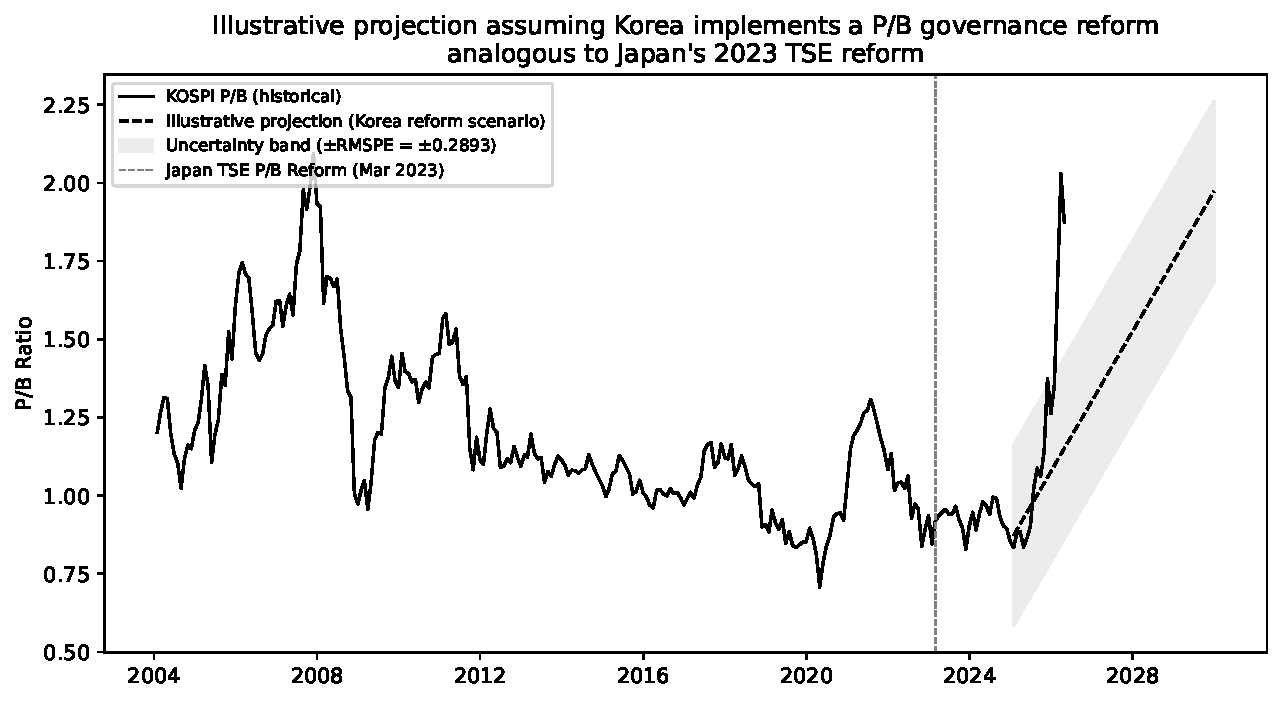
\includegraphics[width=\textwidth]{../output/figures/figure4_counterfactual_projection.pdf}
  \caption{Illustrative projection of KOSPI P/B assuming Korea implements a P/B governance reform analogous to Japan's 2023 TSE reform.}
  \label{fig:counterfactual}
\end{figure}

\bibliographystyle{apalike}
\bibliography{references}

\begin{appendices}

\section{Variable Definitions}
% APPENDIX A -- to be completed in Plan 04

\section{Additional Robustness Tables}
% APPENDIX B -- to be completed in Plan 04

% Figure: Geopolitical risk overlay
\begin{figure}[htbp]
  \centering
  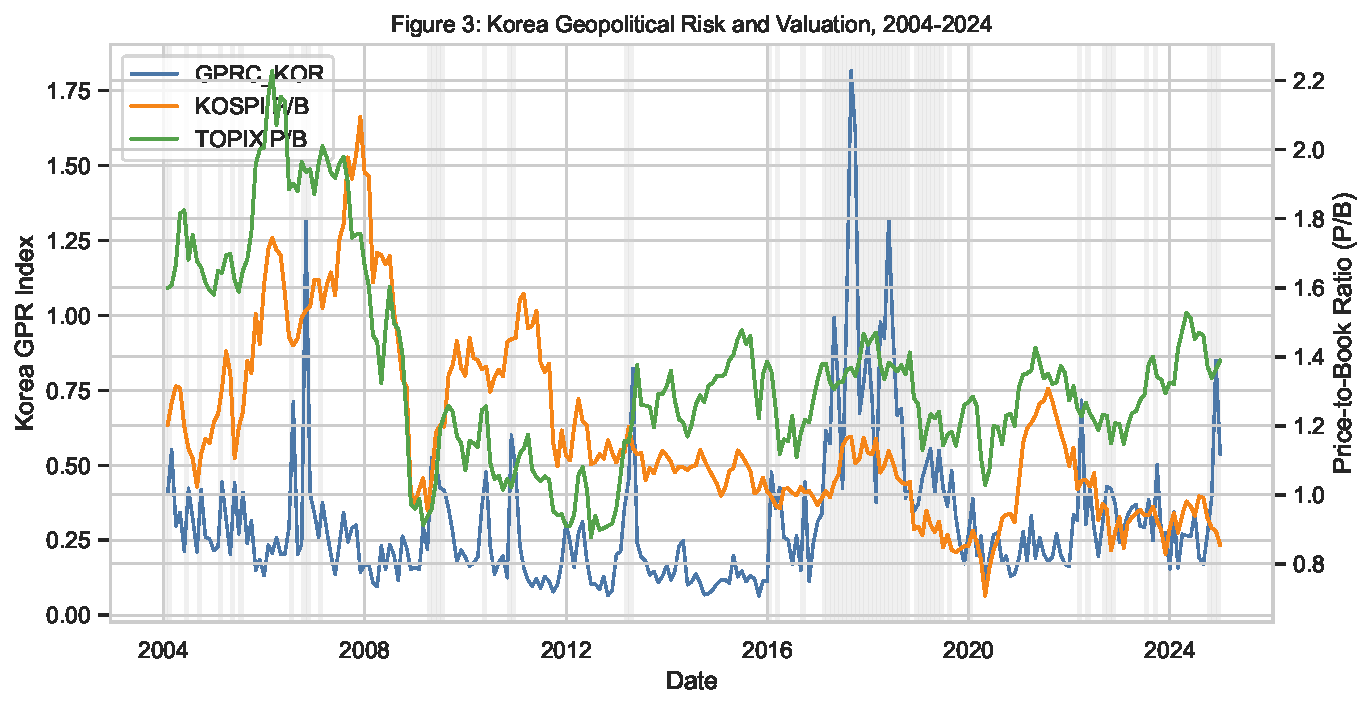
\includegraphics[width=\textwidth]{../output/figures/figure3_geo_risk.pdf}
  \caption{Geopolitical risk index (GPR) and KOSPI P/B discount.}
  \label{fig:geo_risk}
\end{figure}

% Table 3: Geopolitical risk regression
% Geo-risk regression table - auto-generated by geo_risk.py
\begin{table}[htbp]
\centering
\caption{Korea Geopolitical Risk and KOSPI Valuation}
\begin{tabular}{lrrrr}
\toprule
Term & Estimate & Std. Error & t-stat & p-value \\
\midrule
GPR escalation dummy & -0.02 & 0.02 & -0.84 & 0.40 \\
TOPIX P/B & 0.63 & 0.12 & 5.40 & 0.00 \\
\bottomrule
\end{tabular}
\begin{flushleft}\footnotesize N = 252 monthly observations. Year fixed effects included. GPR escalation threshold = 0.37. Partial identification caveat: the GPR-Korea escalation coefficient is an association, not a pure causal effect, because GPRC_KOR may also capture global risk-off episodes.\end{flushleft}
\end{table}


% Synthetic control gap plot
\begin{figure}[htbp]
  \centering
  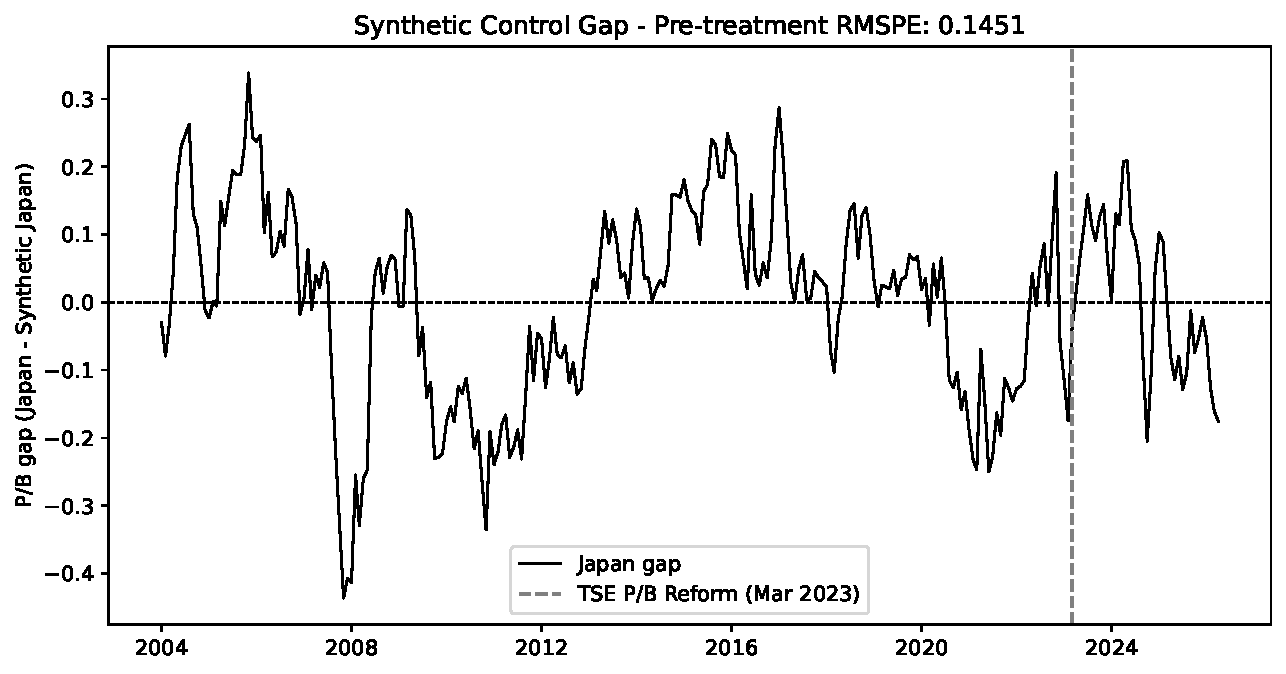
\includegraphics[width=\textwidth]{../output/figures/figure_synth_gap.pdf}
  \caption{Synthetic control gap: TOPIX P/B (actual) minus synthetic TOPIX P/B, 2023 TSE P/B reform.}
  \label{fig:synth_gap}
\end{figure}

% Robustness table fragments
\begin{table}
\caption{Panel OLS Robustness - EM ASIA Control Group}
\label{tab:robust_alt_em_asia}
\begin{tabular}{llll}
\toprule
 & Baseline two-way FE & + reform dummies & + reform x Japan \\
term &  &  &  \\
\midrule
Post Stewardship Code &  & absorbed by time FE & absorbed by time FE \\
Post Corporate Governance Code &  & absorbed by time FE & absorbed by time FE \\
Post TSE P/B Reform &  & absorbed by time FE & absorbed by time FE \\
Stewardship x Japan &  &  & -0.01 (0.03) \\
Corporate Governance Code x Japan &  &  & -0.28 (0.04) \\
TSE P/B Reform x Japan &  &  & -0.24 (0.12) \\
\multicolumn{4}{l}{\footnotesize Note: Coefficients from two-way FE PanelOLS using robust standard errors in parentheses. Post reform dummies are absorbed by time fixed effects where noted.} \\
\bottomrule
\end{tabular}
\end{table}

\input{../output/robustness/robustness_alt_control_em_exchina.tex}
\begin{table}
\caption{P/E robustness: two-way fixed effects PanelOLS estimates of Japan reform valuation responses.}
\label{tab:robustness_pe_panel_ols}
\begin{tabular}{llll}
\toprule
 & Baseline two-way FE & + reform dummies & + reform x Japan \\
term &  &  &  \\
\midrule
post\_stewardship &  & absorbed by time FE & absorbed by time FE \\
post\_cgc &  & absorbed by time FE & absorbed by time FE \\
post\_tse\_pb\_reform &  & absorbed by time FE & absorbed by time FE \\
stewardship\_x\_japan &  &  & -32.08 [0.125] \\
cgc\_x\_japan &  &  & -0.09 [0.875] \\
tse\_pb\_reform\_x\_japan &  &  & -0.47 [0.250] \\
\multicolumn{4}{l}{\footnotesize Note: Coefficients use P/E (price-to-earnings) as the dependent variable in two-way FE PanelOLS. For \textit{+ reform x Japan} specification, bracketed values are wild-bootstrap p-values (999 Rademacher draws, clustered by country). Standard errors shown for all other estimable cells.} \\
\bottomrule
\end{tabular}
\end{table}

% P/E robustness descriptive CARs: coefficients and cumulative abnormal KOSPI-TOPIX P/E spread.
% Standard errors are not reported: the saturated cohort x relative-time design
% makes sandwich robust inference undefined. See paper text for robustness discussion.
\begin{table}
\caption{P/E stacked event-study descriptive CAR estimates (no inference reported).}
\label{tab:robustness_pe_event_study_coefs}
\begin{tabular}{lrrr}
\toprule
Event & Month & Coefficient & CAR \\
\midrule
Japan Stewardship Code (Feb 2014) & -12 & -5.80 & -5.80 \\
Japan Stewardship Code (Feb 2014) & -11 & -3.27 & -9.07 \\
Japan Stewardship Code (Feb 2014) & -10 & -1.71 & -10.78 \\
Japan Stewardship Code (Feb 2014) & -9 & -4.39 & -15.17 \\
Japan Stewardship Code (Feb 2014) & -8 & 0.25 & -14.92 \\
Japan Stewardship Code (Feb 2014) & -7 & -0.60 & -15.52 \\
Japan Stewardship Code (Feb 2014) & -6 & -0.28 & -15.80 \\
Japan Stewardship Code (Feb 2014) & -5 & 3.15 & -12.66 \\
Japan Stewardship Code (Feb 2014) & -4 & 2.43 & -10.22 \\
Japan Stewardship Code (Feb 2014) & -3 & 2.78 & -7.44 \\
Japan Stewardship Code (Feb 2014) & -2 & 3.28 & -4.16 \\
Japan Stewardship Code (Feb 2014) & -1 & 0.00 & -4.16 \\
Japan Stewardship Code (Feb 2014) & 0 & 3.20 & -0.96 \\
Japan Stewardship Code (Feb 2014) & 1 & 2.39 & 1.43 \\
Japan Stewardship Code (Feb 2014) & 2 & 5.72 & 7.15 \\
Japan Stewardship Code (Feb 2014) & 3 & 5.70 & 12.85 \\
Japan Stewardship Code (Feb 2014) & 4 & 10.02 & 22.88 \\
Japan Stewardship Code (Feb 2014) & 5 & 9.37 & 32.25 \\
Japan Stewardship Code (Feb 2014) & 6 & 9.87 & 42.12 \\
Japan Stewardship Code (Feb 2014) & 7 & 8.92 & 51.03 \\
Japan Stewardship Code (Feb 2014) & 8 & 7.82 & 58.85 \\
Japan Stewardship Code (Feb 2014) & 9 & 7.28 & 66.14 \\
Japan Stewardship Code (Feb 2014) & 10 & 13.07 & 79.20 \\
Japan Stewardship Code (Feb 2014) & 11 & 12.64 & 91.84 \\
Japan Stewardship Code (Feb 2014) & 12 & 13.20 & 105.04 \\
Japan Stewardship Code (Feb 2014) & 13 & -0.53 & 104.51 \\
Japan Stewardship Code (Feb 2014) & 14 & 2.64 & 107.15 \\
Japan Stewardship Code (Feb 2014) & 15 & 2.91 & 110.07 \\
Japan Stewardship Code (Feb 2014) & 16 & 1.70 & 111.77 \\
Japan Stewardship Code (Feb 2014) & 17 & 2.16 & 113.94 \\
Japan Stewardship Code (Feb 2014) & 18 & 1.38 & 115.31 \\
Japan Stewardship Code (Feb 2014) & 19 & 3.37 & 118.68 \\
Japan Stewardship Code (Feb 2014) & 20 & 4.79 & 123.48 \\
Japan Stewardship Code (Feb 2014) & 21 & 3.82 & 127.30 \\
Japan Stewardship Code (Feb 2014) & 22 & 3.82 & 131.12 \\
Japan Stewardship Code (Feb 2014) & 23 & 3.89 & 135.01 \\
Japan Stewardship Code (Feb 2014) & 24 & 4.64 & 139.65 \\
TSE Corporate Governance Code (Jun 2015) & -12 & 4.77 & 4.77 \\
TSE Corporate Governance Code (Jun 2015) & -11 & 3.82 & 8.60 \\
TSE Corporate Governance Code (Jun 2015) & -10 & 4.02 & 12.61 \\
TSE Corporate Governance Code (Jun 2015) & -9 & 2.76 & 15.38 \\
TSE Corporate Governance Code (Jun 2015) & -8 & 1.37 & 16.74 \\
TSE Corporate Governance Code (Jun 2015) & -7 & 0.53 & 17.27 \\
TSE Corporate Governance Code (Jun 2015) & -6 & 6.01 & 23.28 \\
TSE Corporate Governance Code (Jun 2015) & -5 & 5.28 & 28.56 \\
TSE Corporate Governance Code (Jun 2015) & -4 & 5.54 & 34.09 \\
TSE Corporate Governance Code (Jun 2015) & -3 & -8.49 & 25.60 \\
TSE Corporate Governance Code (Jun 2015) & -2 & -5.62 & 19.98 \\
TSE Corporate Governance Code (Jun 2015) & -1 & 0.00 & 19.98 \\
TSE Corporate Governance Code (Jun 2015) & 0 & -7.16 & 12.82 \\
TSE Corporate Governance Code (Jun 2015) & 1 & -7.00 & 5.82 \\
TSE Corporate Governance Code (Jun 2015) & 2 & -8.09 & -2.27 \\
TSE Corporate Governance Code (Jun 2015) & 3 & -6.40 & -8.67 \\
TSE Corporate Governance Code (Jun 2015) & 4 & -5.28 & -13.95 \\
TSE Corporate Governance Code (Jun 2015) & 5 & -6.55 & -20.50 \\
TSE Corporate Governance Code (Jun 2015) & 6 & -6.85 & -27.35 \\
TSE Corporate Governance Code (Jun 2015) & 7 & -7.09 & -34.44 \\
TSE Corporate Governance Code (Jun 2015) & 8 & -6.64 & -41.07 \\
TSE Corporate Governance Code (Jun 2015) & 9 & -9.34 & -50.41 \\
TSE Corporate Governance Code (Jun 2015) & 10 & -7.04 & -57.45 \\
TSE Corporate Governance Code (Jun 2015) & 11 & -7.25 & -64.70 \\
TSE Corporate Governance Code (Jun 2015) & 12 & -9.12 & -73.82 \\
TSE Corporate Governance Code (Jun 2015) & 13 & -7.84 & -81.67 \\
TSE Corporate Governance Code (Jun 2015) & 14 & -8.62 & -90.28 \\
TSE Corporate Governance Code (Jun 2015) & 15 & -10.03 & -100.32 \\
TSE Corporate Governance Code (Jun 2015) & 16 & -10.19 & -110.50 \\
TSE Corporate Governance Code (Jun 2015) & 17 & -11.59 & -122.09 \\
TSE Corporate Governance Code (Jun 2015) & 18 & -13.86 & -135.95 \\
TSE Corporate Governance Code (Jun 2015) & 19 & -14.41 & -150.37 \\
TSE Corporate Governance Code (Jun 2015) & 20 & -14.45 & -164.82 \\
TSE Corporate Governance Code (Jun 2015) & 21 & -17.79 & -182.60 \\
TSE Corporate Governance Code (Jun 2015) & 22 & -15.51 & -198.12 \\
TSE Corporate Governance Code (Jun 2015) & 23 & -15.00 & -213.11 \\
TSE Corporate Governance Code (Jun 2015) & 24 & -13.43 & -226.54 \\
TSE P/B Reform Request (Mar 2023) & -12 & -1.42 & -1.42 \\
TSE P/B Reform Request (Mar 2023) & -11 & 0.38 & -1.05 \\
TSE P/B Reform Request (Mar 2023) & -10 & 0.65 & -0.39 \\
TSE P/B Reform Request (Mar 2023) & -9 & 0.80 & 0.41 \\
TSE P/B Reform Request (Mar 2023) & -8 & -0.20 & 0.21 \\
TSE P/B Reform Request (Mar 2023) & -7 & 0.04 & 0.25 \\
TSE P/B Reform Request (Mar 2023) & -6 & -1.07 & -0.82 \\
TSE P/B Reform Request (Mar 2023) & -5 & -1.26 & -2.08 \\
TSE P/B Reform Request (Mar 2023) & -4 & -1.18 & -3.25 \\
TSE P/B Reform Request (Mar 2023) & -3 & 0.48 & -2.77 \\
TSE P/B Reform Request (Mar 2023) & -2 & 0.25 & -2.52 \\
TSE P/B Reform Request (Mar 2023) & -1 & 0.00 & -2.52 \\
TSE P/B Reform Request (Mar 2023) & 0 & -0.26 & -2.78 \\
TSE P/B Reform Request (Mar 2023) & 1 & 1.11 & -1.67 \\
TSE P/B Reform Request (Mar 2023) & 2 & 1.02 & -0.65 \\
TSE P/B Reform Request (Mar 2023) & 3 & 4.30 & 3.65 \\
TSE P/B Reform Request (Mar 2023) & 4 & 3.37 & 7.02 \\
TSE P/B Reform Request (Mar 2023) & 5 & 3.63 & 10.65 \\
TSE P/B Reform Request (Mar 2023) & 6 & 7.61 & 18.26 \\
TSE P/B Reform Request (Mar 2023) & 7 & 7.20 & 25.46 \\
TSE P/B Reform Request (Mar 2023) & 8 & 6.68 & 32.13 \\
TSE P/B Reform Request (Mar 2023) & 9 & 8.13 & 40.26 \\
TSE P/B Reform Request (Mar 2023) & 10 & 9.23 & 49.49 \\
TSE P/B Reform Request (Mar 2023) & 11 & 7.22 & 56.71 \\
TSE P/B Reform Request (Mar 2023) & 12 & 9.28 & 65.99 \\
TSE P/B Reform Request (Mar 2023) & 13 & 9.81 & 75.80 \\
TSE P/B Reform Request (Mar 2023) & 14 & 9.84 & 85.64 \\
TSE P/B Reform Request (Mar 2023) & 15 & 6.37 & 92.01 \\
TSE P/B Reform Request (Mar 2023) & 16 & 7.40 & 99.42 \\
TSE P/B Reform Request (Mar 2023) & 17 & 7.50 & 106.91 \\
TSE P/B Reform Request (Mar 2023) & 18 & 6.13 & 113.04 \\
TSE P/B Reform Request (Mar 2023) & 19 & 6.30 & 119.34 \\
TSE P/B Reform Request (Mar 2023) & 20 & 6.00 & 125.34 \\
TSE P/B Reform Request (Mar 2023) & 21 & 5.64 & 130.98 \\
TSE P/B Reform Request (Mar 2023) & 22 & 5.01 & 136.00 \\
TSE P/B Reform Request (Mar 2023) & 23 & 5.71 & 141.71 \\
TSE P/B Reform Request (Mar 2023) & 24 & 6.76 & 148.47 \\
\bottomrule
\end{tabular}
\end{table}


\end{appendices}

\end{document}
